%versi 2 (8-10-2016)
\chapter{Landasan Teori}
\label{chap:teori}

Pada bab ini akan dibahas mengenai dasar-dasar teori yang dipakai dalam skripsi ini. Teori di dalam bab ini dimulai dengan \textit{Outlook Calendar} yang merupakan suatu aplikasi yang dipakai untuk menyimpan data \textit{event}, lalu di dalam \textit{Outlook Calendar} akan dibahas mengenai \textit{API} yang telah disediakan oleh \textit{Windows Live}. Lalu setelah membahas mengenai \textit{Outlook Calendar}, dilanjutkan dengan membahas mengenai \textit{Slack} beserta \textit{API} yang telah disediakan oleh \textit{Slack}. Dilanjutkan dengan membahas mengenai \textit{Node.js} yang merupakan sebuah \textit{platform} yang digunakan untuk membangun perangkat lunak skripsi ini, serta akan membahas mengenai \textit{library-library} yang dipakai untuk membangun skripsi ini. Setelah itu akan membahas mengenai \textit{Heroku} yang merupakan sebuah \textit{cloud platform} yang memiliki fungsi seperti layaknya \textit{server} yang digunakan untuk melakukan \textit{hosting} dari berbagai perangkat lunak. 

\section{Outlook Calendar}
\textit{Outlook calendar} adalah aplikasi yang tergabung dalam layanan dari \textit{Microsoft} yang memiliki fungsi sebagai kalender. Layanan ini bisa terhubung dengan aplikasi lainnya dengan menggunakan \textit{API} yang telah dibuat dan disediakan oleh pihak \textit{Microsoft}, yaitu yang terkumpul di dalam \textit{Microsoft Graph API}. Maksud dari \textit{API} adalah \textit{interface} yang memungkinkan 2 aplikasi atau lebih untuk saling berinteraksi. Umumnya cara kerja dari \textit{API} adalah dengan mengirimkan \textit{request} bertipe \textit{get} atau \textit{post} kepada sebuah \textit{endpoint} tertentu dengan \textit{parameter} yang dibutuhkan oleh \textit{API} tersebut. \textit{Endpoint} adalah alamat tujuan yang pada umumnya sudah disediakan oleh penyedia \textit{API}, sedangkan \textit{parameter} merupakan masukan yang diperlukan oleh fungsi \textit{API} itu sendiri. Pembahasan tentang \textit{Microsoft Graph API} akan dibahas pada bagian subsubbab \ref{sec:microsoftgraph} 

\subsection{\textit{Microsoft Graph API}}
\label{sec:microsoftgraph}
\textit{Microsoft Graph API} adalah \textit{API} yang berguna untuk mendapatkan data-data yang terdapat di dalam layanan \textit{Microsoft} 365 yaitu seperti \textit{Azure Active Directory}, layanan \textit{Office} 365 (\textit{SharePoint, OneDrive, Outlook/Exchange, Microsoft Teams, OneNote, Planner,} dan \textit{Excel}), layanan \textit{Enterprise Mobility and Security} (\textit{Identity Manager, Intune, Advanced Threat Analytics,} dan \textit{Advanced Threat Protection}), layanan \textit{Windows} 10 (\textit{activities} dan \textit{devices}), dan \textit{Education}. Terdapat 2 versi referensi untuk \textit{Microsoft Graph API} yaitu versi 1.0 dan juga versi beta, tetapi yang dituliskan pada subsubbab ini mengacu kepada versi 1.0. \cite{microsoft} Pada versi 1.0, \textit{endpoint} utama yang dipakai akan mengacu kepada \textit{endpoint} \textit{https://graph.microsoft.com/v1.0}. 

Untuk menggunakan fungsi dari \textit{Microsoft Graph API}, dibutuhkan untuk mendaftarkan aplikasi yang akan dirancang dan memakai fungsi dari \textit{API} dari \textit{Microsoft Graph API} ke \textit{Microsoft App Registration Portal}\footnote{https://apps.dev.microsoft.com/}. Pada saat mendaftarkan aplikasinya, akan didapatkan \textit{application ID} yang adalah pengenal unik untuk aplikasi yang didaftarkan, dan juga \textit{Redirect URL} yang didaftarkan sebagai \textit{URL} yang akan menerima kembalian \textit{authentication} dan \textit{token} yang akan dikirim oleh \textit{endpoint Azure AD v2.0}, serta mendapat \textit{application secret} yang didapat saat mengklik ``\textit{Generate New Password}'' saat mendaftarkan aplikasi (berlaku jika mendaftarkan aplikasi berjenis \textit{web apps}). \textit{Application ID} yang didapat saat mendaftar aplikasi akan dipakai untuk mengisi nilai dari parameter \textit{client\_id} yang akan diisi pada saat akan mengirimkan \textit{request} untuk mendapatkan \textit{authorization\_code}. Setelah mendapatkan \textit{authorization\_code}, maka langkah selanjutnya adalah meminta \textit{access\_token} yang membutuhkan \textit{parameter} \textit{authorization\_code} kepada \textit{field code}, dan juga \textit{application\_secret} yang didapat dari pendaftaran aplikasi sebelumnya yang akan mengisi \textit{field client\_secret}. \textit{Response} dari \textit{request token} akan mengembalikkan jangka waktu aktif dari \textit{token} tersebut dan juga \textit{refresh\_token} yang akan berguna untuk meminta \textit{refresh\_token} saat \textit{token} sudah \textit{expired}.

Setelah mendapatkan \textit{access token}, layanan untuk mendapatkan dan memanipulasi data yang tersimpan di \textit{Microsoft} baru bisa diakses. Ada banyak layanan yang disediakan dari \textit{Microsoft Graph API} yang tergolong di dalam \textit{resource type}. \textit{Resource type} merupakan kelas yang representasi dari objek yang disimpan oleh \textit{Microsoft}. Berikut beberapa \textit{resource type} yang disediakan oleh \textit{Microsoft}:

\subsubsection{User resource type}
Kelas \textit{user} ini merepresentasikan \textit{Azure AD user account}. Kelas ini memiliki properti-properti dan juga \textit{method-method}:\\

\subsubsubsection{Properti}
\begin{itemize}
	\item \textbf{\textit{aboutMe}}\\
	Properti ini bertipe \textit{String} yang merupakan \textit{field} untuk mendeskripsikan diri pengguna. 
	\item \textbf{\textit{accountEnabled}}\\
	Properti ini bertipe \textit{Boolean} yang bernilai \textbf{\textit{true}} jika akun diaktifkan dan akan bernilai \textbf{\textit{false}} jika tidak. Properti ini berguna saat akan membuat akun. Nilai ini yang akan dipakai sebagai patokan sebuah akun bisa dibuat atau tidaknya. 
	\item \textbf{\textit{ageGroup}}\\
	Properti ini bertipe \textit{String} yang merupakan nilai kelompok umur dari pengguna. Terdapat nilai \textbf{\textit{null}}, \textbf{\textit{minor}}, \textbf{\textit{notAdult}}, dan juga \textbf{\textit{adult}}.
	\item \textbf{\textit{assignedLicenses}}\\
	Properti ini bertipe koleksi \textit{assignedLicense} yang merupakan nilai lisensi yang diberikan kepada pengguna.
	\item \textbf{\textit{assignedPlans}}\\
	Properti ini bertipe koleksi \textit{assignedPlan} yang merupakan nilai \textit{plan} yang diberikan kepada pengguna.
	\item \textbf{\textit{birthday}}\\
	Properti ini bertipe \textit{DateTimeOffset} yang merupakan nilai ulang tahun dari pengguna. 
	\item \textbf{\textit{businessPhones}}\\
	Properti ini bertipe \textit{String} yang merupakan nomor telepon dari pengguna. Walaupun bersifat \textit{String}, tetapi \textit{field} ini hanya bisa diisi oleh angka.
	\item \textbf{\textit{city}}\\
	Properti ini bertipe \textit{String} yang merupakan kota lokasi pengguna.
	\item \textbf{\textit{companyName}}\\
	Properti ini bertipe \textit{String} yang merupakan nama perusahaan dimana pengguna terkait di dalamnya.
	\item \textbf{\textit{consentProvidedForMinor}}\\
	Properti ini bertipe \textit{String} yang merupakan status persetujuan bagi anak dibawah umur yang mengacu kepada properti \textit{ageGroup}. Nilai dari properti ini bisa \textbf{\textit{null}}, \textbf{\textit{granted}}, \textbf{\textit{denied}}, dan juga \textbf{\textit{notRequired}}. 
	\item \textbf{\textit{country}}\\
	Properti ini bertipe \textit{String} yang merupakan negara lokasi pengguna.
	\item \textbf{\textit{createDateTime}}\\
	Properti ini bertipe \textit{DateTimeOffset} yang merupakan tanggal dibuatnya objek pengguna.
	\item \textbf{\textit{department}}\\
	Properti ini bertipe \textit{String} yang merupakan nama departemen pengguna bekerja.
	\item \textbf{\textit{displayName}}\\
	Properti ini bertipe \textit{String} yang merupakan nama yang ditampilkan di buku alamat untuk pengguna. Biasanya disusun dari nama depan, nama tengah, dan juga nama belakang. Properti ini merupakan properti yang \textit{required} ketika pengguna dibuat dan tidak bisa dihapus. 
	 \item \textbf{\textit{employeeId}}\\
	Properti ini bertipe \textit{String} yang merupakan pengidentifikasi karyawan yang diberikan kepada pengguna oleh organisasi.
	\item \textbf{\textit{faxNumber}}\\
	Properti ini bertipe \textit{String} yang merupakan nomor fax pengguna.
	\item \textbf{\textit{givenName}}\\
	Properti ini bertipe \textit{String} yang merupakan nama depan dari pengguna.
	\item \textbf{\textit{hireDate}}\\
	Properti ini bertipe \textit{DateTimeOffset} yang merupakan tanggal pengguna dipekerjakan.
	\item \textbf{\textit{id}}\\
	Properti ini bertipe \textit{String} yang merupakan tanda pengenal unik untuk pengguna.
	\item \textbf{\textit{imAddresses}}\\
	Properti ini bertipe koleksi \textit{String} yang merupakan alamat protokol inisiasi sesi \textit{voice over IP} (VOIP) pesan untuk pengguna.
	\item \textbf{\textit{interests}}\\
	Properti ini bertipe koleksi \textit{String} yang merupakan kumpulan \textit{String} yang mendeskripsikan ketertarikan dari pengguna.
	\item \textbf{\textit{isResourceAccount}}\\
	Properti ini bertipe \textit{Boolean} yang akan bernilai \textbf{\textit{true}} jika akun merupakan \textit{resource account} dan akan bernilai \textbf{\textit{false}} jika bukan. Jika kosong akan dianggap dengan nilai \textit{false}.
	\item \textbf{\textit{jobTitle}}\\
	Properti ini bertipe \textit{String} yang merupakan jabatan dari pengguna.
	\item \textbf{\textit{legalAgeGroupClassification}}
	Properti ini bertipe \textit{String} yang merupakan penentu kelompok \textit{legalAge} dengan dihitung menggunakan properti \textit{ageGroup} dan juga \textit{consentProvidedForMinor}. Nilai dari properti ini bisa berupa \textit{null}, \textit{minorWithOutParentalConsent}, \textit{minorWithParentalConsent}, \textit{minorNoParentalConsentRequired}, \textit{notAdult}, dan juga \textit{adult}. Properti ini bersifat \textbf{\textit{Read-Only}}.
	 \item \textbf{\textit{licenseAssignmentStates}}\\
	Properti ini bertipe koleksi \textit{licenseAssignmentState} yang merupakan status penugasan lisensi untuk pengguna. Properti ini bersifat \textbf{\textit{Read-Only}}.
	\item \textbf{\textit{mail}}\\
	Properti ini bertipe \textit{String} yang merupakan alamat SMTP untuk pengguna. Properti ini bersifat \textbf{\textit{Read-Only}}.
	\item \textbf{\textit{mailboxSettings}}\\
	Properti ini bertipe \textit{mailboxSettings} yang merupakan pengaturan untuk \textit{mailbox} utama dari pengguna yang masuk.
	\item \textbf{\textit{mailNickname}}\\
	Properti ini bertipe \textit{String} yang merupakan alias \textit{email} dari pengguna. Properti ini harus ditentukan saat pengguna dibuat. 
	\item \textbf{\textit{mobilePhone}}\\
	Properti ini bertipe \textit{String} yang merupakan nomor telepon seluler utama pengguna.
	\item \textbf{\textit{mySite}}\\
	Properti ini bertipe \textit{String} yang merupakan \textit{url} untuk situs pribadi pengguna.
	\item \textbf{\textit{officeLocation}}\\
	Properti ini bertipe \textit{String} yang merupakan lokasi kantor di tempat bisnis pengguna.
	\item \textbf{\textit{onPremisesDistinguishedName}}\\
	Properti ini bertipe \textit{String} yang merupakan nama atau DN Direktori Aktif lokal yang dibedakan. Properti ini hanya diisi untuk pelanggan yang menyinkronkan direktori lokal mereka ke \textit{Azure Active Directory} melalui \textit{Azure AD Connect}. Properti ini bersifat \textbf{\textit{Read-Only}}.
	\item \textbf{\textit{onPremisesDomainName}}\\
	Properti ini bertipe \textit{String} yang merupakan \textit{dnsDomainName} yang disinkronkan dari direktori lokal. Properti ini hanya diisi untuk pelanggan yang menyinkronkan direktori lokal mereka ke \textit{Azure Active Directory} melalui \textit{Azure AD Connect}. Properti ini bersifat \textbf{\textit{Read-Only}}.
	\item \textbf{\textit{onPremisesExtensionAttributes}}\\
	Properti ini bertipe \textit{OnPremisesExtensionAttributes} yang merupakan \textit{extensionAttributes} untuk pengguna. Jika properti \textit{onPremisesSyncEnabled} bernilai \textbf{\textit{true}}, maka properti ini bersifat \textbf{\textit{Read-Only}}, tetapi jika properti \textit{onPremisesSyncEnabled} bernilai \textbf{\textit{false}}, maka properti ini dapat diatur saat membuat atau memperbarui.
	\item \textbf{\textit{onPremisesImmutableId}}\\
	Properti ini bertipe \textit{String} yang digunakan untuk mengaitkan akun pengguna \textit{Active Directory} lokal ke objek \textit{Azure AD} pengguna. Properti ini ditentukan saat pembuatan akun pengguna baru di \textit{Graph}.
	\item \textbf{onPremisesLastSyncDateTime}\\
	Properti ini bertipe DateTimeOffset yang memiliki fungsi untuk menunjukkan kapan terakhir kali objek disinkronkan dengan direktori lokal. Properti ini bersifat \textbf{\textit{Read-Only}}. 
	\item \textbf{\textit{onPremisesProvisioningErrors}}\\
	Properti ini bertipe koleksi \textit{onPremisesProvisioningError} yang merupakan kesalahan saat menggunakan produk sinkronisasi \textit{Microsoft}.
	 \item \textbf{\textit{onPremisesSamAccountName}}\\
	Properti ini bertipe \textit{String} yang merupakan \textit{samAccountName} lokal yang disinkronkan dari direktori lokal. Properti ini hanya diisi untuk pelanggan yang menyinkronkan direktori lokal mereka ke \textit{Azure Active Directory} melalui \textit{Azure AD Connect}. Properti ini bersifat \textbf{\textit{Read-Only}}.
	\item \textbf{\textit{onPremisesSecurityIdentifier}}\\
	Properti ini bertipe \textit{String} yang merupakan pengidentifikasi keamanan lokal (SID) untuk pengguna yang disinkronkan dari lokal ke \textit{cloud}. Properti ini bersifat \textbf{\textit{Read-Only}}.
	\item \textbf{\textit{onPremisesSyncEnabled}}\\
	Properti ini bertipe \textit{Boolean} yang bernilai \textbf{\textit{true}} jika objek ini disinkronisasi dari direktori lokal dan bernilai \textbf{\textit{false}} jika objek ini awalnya disinkronisasi dari direktori lokal tetapi tidak lagi disinkronkan. Properti ini juga bisa bernilai \textbf{\textit{null}} jika objek ini tidak pernah disinkronkan dari direktori lokal. Properti ini bersifat \textbf{\textit{Read-Only}}.
	\item \textbf{\textit{onPremisesUserPrincipalName}}\\
	Properti ini bertipe \textit{String} yang merupakan \textit{userPrincipalName} di tempat yang disinkronkan dari direktori lokal. Properti ini hanya diisi untuk pelanggan yang menyinkronkan direktori lokal mereka ke \textit{Azure Active Directory} melalui \textit{Azure AD Connect}. Properti ini bersifat \textbf{\textit{Read-Only}}.
	\item \textbf{\textit{otherMails}}\\
	Properti ini bertipe \textit{String} yang merupakan daftar dari alamat \textit{email} tambahan untuk pengguna.
	\item \textbf{\textit{passwordPolicies}}\\
	Properti ini bertipe \textit{String} yang menentukan kebijakan kata sandi untuk pengguna. 
	\item \textbf{\textit{passwordProfile}}\\
	Properti ini bertipe \textit{passwordProfile} yang menentukan profil kata sandi untuk pengguna. Profil ini berisi kata sandi dari pengguna. Properti ini diperlukan saat pengguna dibuat dan kata sandi harus memenuhi persyaratan yang ditentukan oleh properti \textit{passswordPolicies}.
	\item \textbf{\textit{pastProjects}}\\
	Properti ini bertipe koleksi \textit{String} yang merupakan daftar proyek yang sudah lalu dari pengguna.
	\item \textbf{\textit{postalCode}}\\
	Properti ini bertipe \textit{String} yang merupakan kode pos dari pengguna.
	\item \textbf{\textit{preferredDataLocation}}\\
	Properti ini bertipe \textit{String} yang merupakan lokasi data yang dipilih oleh pengguna.
	 \item \textbf{\textit{preferredLanguage}}\\
	Properti ini bertipe \textit{String} yang merupakan bahasa yang dipilih oleh pengguna.
	\item \textbf{\textit{preferredName}}\\
	Properti ini bertipe \textit{String} yang merupakan nama yang dipilih oleh pengguna.
	\item \textbf{\textit{provisionedPlans}}\\
	Properti ini bertipe koleksi \textit{provisionedPlan} yang merupakan \textit{plan} yang disediakan untuk pengguna. Properti ini bersifat \textbf{\textit{Read-Only}} dan tidak bisa bernilai \textbf{\textit{null}}.
	\item \textbf{\textit{proxyAddresses}}\\
	Properti ini bertipe koleksi \textit{String}.
	\item \textbf{\textit{responsibilities}}\\
	Properti ini bertipe koleksi \textit{String} yang merupakan daftar dari tanggung jawab pengguna.
	\item \textbf{\textit{schools}}\\
	Properti ini bertipe koleksi \textit{String} yang merupakan daftar dari instansi pendidikan yang pernah dihadiri oleh pengguna.
	\item \textbf{\textit{showInAddressList}}\\
	Properti ini bertipe \textit{Boolean} yang bernilai \textbf{\textit{true}} jika daftar alamat \textit{Outlook global} harus berisi pengguna ini, dan bernilai \textbf{\textit{false}} jika tidak. Jika tidak diberikan nilai, maka akan bernilai \textbf{\textit{true}}. 
	\item \textbf{\textit{skills}}\\
	Properti ini bertipe koleksi \textit{String} yang merupakan daftar dari kemampuan pengguna. 
	\item \textbf{\textit{state}}\\
	Properti ini bertipe \textit{String} yang merupakan negara atau provinsi yang terdapat di alamat pengguna. 
	\item \textbf{\textit{streetAddress}}\\
	Properti ini bertipe \textit{String} yang merupakan alamat dari tempat bisnis pengguna.
	\item \textbf{\textit{surname}}\\
	Properti ini bertipe \textit{String} yang merupakan nama keluarga atau nama belakang dari pengguna.  
	\item \textbf{\textit{usageLocation}}\\
	Properti ini bertipe \textit{String} yang merupakan 2 huruf dari kode negara pengguna yang digunakan untuk memeriksa ketersediaan layanan di negara pengguna. 
	\item \textbf{\textit{userPrincipalName}}\\
	Properti ini bertipe \textit{String} yang merupakan nama utama dari pengguna yang memakai standar internet RFC 822.
	\item \textbf{\textit{userType}}\\
	Properti ini bertipe \textit{String} yang digunakan untuk mengklasifikasi tipe pengguna, seperti contohnya ``\textit{Member}'' dan ``\textit{Guest}''.	 
\end{itemize}

\subsubsubsection{Method}\\
Untuk mengakses setiap \textit{method} yang dijabarkan, perlu diketahui bahwa untuk mengirimkan \textit{request}, diperlukan \textit{header} yang berisikan \textit{Authorization} yang diisi dengan nilai dari \textit{Access\_token} yang didapat dari proses permintaan \textit{access token}. \textit{Endpoint} utama untuk mengirimkan request adalah ke \textit{https://graph.microsoft.com/v1.0} lalu dilanjutkan dengan \textit{endpoint} fungsinya masing-masing seperti yang diberikan dan dijelaskan. 

\begin{itemize}
	\item \textbf{\textit{List users}}\\
	\textit{Method} ini berfungsi untuk mendapatkan daftar dari objek pengguna. \textit{Method} ini di\textit{request} dengan cara mengirim \textit{request} \textit{get} kepada \textit{endpoint} \textit{/users} dengan \textit{headers} berisikan otorisasi yang diisi dengan nilai dari \textit{access token} dan juga \textit{Content-Type} yang bernilai \textit{application/json}. \textit{Request} untuk \textit{method} ini juga bisa diisi dengan \textit{parameter} \textit{\$select} untuk mengembalikan \textit{field} yang hanya diisi di dalam \textit{parameter} \$select tersebut, dan dalam \textit{parameter} itu, tiap \textit{field} dipisah dengan tanda koma (,) contohnya \textit{https://graph.microsoft.com/v1.0/users?\$select=displayName,givenName,postalCode}.  \textit{Respons} dari method ini akan mengembalikan \textit{json} dari objek pengguna. 
	\item \textbf{\textit{Create user}}\\
	\textit{Method} ini berfungsi untuk membuat pengguna. \textit{Method} ini di\textit{request} dengan cara mengirimkan \textit{request} \textit{post} ke \textit{endpoint} \textit{/users} yang memiliki headers otorisasi yang diisi dengan \textit{access token} dan juga \textit{Content-Type} yang diisi dengan \textit{application/json} dan juga \textit{body} yang berisi \textit{parameter} untuk membuat objek pengguna. \textit{Parameter} yang wajib diisi adalah \textit{accountEnabled, displayName, onPremisesImmutableId, mailNickname, passwordProfile}, dam juga \textit{userPrincipalName}.  
	\item \textbf{\textit{Get user}}\\
	\textit{Method} ini berfungsi untuk membaca properti dan juga hubungan pengguna. \textit{Method} ini di\textit{request} dengan cara mengirim \textit{get request} dan dikirimkan ke \textit{endpoint} \textit{/users/\{id | userPrincipalName\}} atau bisa juga dengan menggunakan \textit{/me} dengan \textit{headers} yang sama dengan \textit{method-method} sebelumnya dan juga bisa menggunakan \textit{parameter} \textit{\$select} seperti \textit{method} sebelumnya.  
	\item \textbf{\textit{Update user}}\\
	\textit{Method} ini berfungsi untuk memperbaharui pengguna. \textit{Method} ini di\textit{request} dengan cara mengirimkan \textit{patch request} kepada \textit{endpoint} \textit{/users/\{id | userPrincipalName\}}. Memiliki \textit{request headers} seperti \textit{method} lainnya dan juga \textit{body} diisi dengan \textit{field} yang akan diubah nilainya. 
	\item \textbf{\textit{Delete user}}\\
	\textit{Method} ini berfungsi untuk menghapus pengguna. \textit{Method} ini diakses dengan mengirimkan \textit{delete request} ke \textit{endpoint} \textit{/users/\{id | userPrincipalName\}}. 
	\item \textbf{\textit{List messages}}\\
	\textit{Method} ini berfungsi untuk mendapatkan semua pesan di kotak surat pengguna yang masuk. \textit{Method} ini diakses dengan cara mengirimkan \textit{get request} ke \textit{endpoint} \textit{/users/\{id | userPrincipalName\}/messages}. 
	\item \textbf{\textit{Create message}}\\
	\textit{Method} ini berfungsi untuk membuat pesan baru untuk dimasukkan ke dalam koleksi pesan. \textit{Method} ini dapat dijalankan dengan cara mengirimkan \textit{post request} ke \textit{endpoint} \textit{/users/\{id|userPrincipalName\}/messages}. \textit{Body} dari \textit{request} ini akan berisi \textit{json} yang merepresentasikan objek \textit{message}. 
	\item \textbf{\textit{List mailFolders}}\\
	\textit{Method} ini berfungsi untuk mendapatkan folder-folder surat dibawah folder \textit{root} dari pengguna yang masuk. \textit{Method} ini dijalankan dengan cara mengirimkan \textit{get request} ke \textit{endpoint} \textit{/users/\{id | userPrincipalName\}/mailFolders}.
	\item \textbf{\textit{Create mailFolder}}\\
	\textit{Method} ini berfungsi untuk membuat \textit{mailFolder} ke dalam koleksi \textit{mailFolders}. \textit{Method} ini dijalankan dengan cara mengirimkan \textit{post request} ke \textit{endpoint} \textit{/users/\{id | userPrincipalName\}/mailFolders}. 
	\item \textbf{\textit{sendMail}}\\
	\textit{Method} ini berfungsi untuk mengirim pesan. \textit{Method} ini dijalankan dengan cara mengirimkan \textit{post request} kepada \textit{endpoint} \textit{/users/\{id | userPrincipalName\}/sendMail}. \textit{Body} dari \textit{request} ini berisi \textit{message} dan juga sebuah \textit{Boolean} untuk atribut \textit{saveToSentItems}.
	\item \textbf{\textit{List events}}\\
	\textit{Method} ini berfungsi untuk mendapatkan daftar objek \textit{event} di dalam kotak pesan dari pengguna. \textit{Method} ini dijalankan dengan cara mengirimkan \textit{get request} kepada \textit{endpoint} \textit{/users/\{id | userPrincipalName\}/events}. \textit{Headers} pada \textit{method} ini akan berisi otorisasi yang diisi nilai dari \textit{access token} sebagai \textit{header} wajib. Lalu ada juga \textit{header} pilihan yaitu \textit{outlook.timezone} dan juga \textit{outlook.body-content-type}. Pada \textit{header timezone}, jika tidak diisi, maka nilai awal yang dikembalikan adalah dalam \textit{UTC}. \textit{Request} ini juga bisa difilter dengan menggunakan \textit{parameter} \textit{\$select}. 
	\item \textbf{\textit{Create event}}\\
	\textit{Method} ini berfungsi untuk membuat \textit{event} ke dalam koleksi dari \textit{event-event}. \textit{Method} ini dijalankan dengan cara mengirimkan \textit{post request} kepada \textit{endpoint} \textit{/users/\{id | userPrincipalName\}/events}. \textit{Body} dari \textit{request} ini akan berisi \textit{json} yang merepresentasikan objek \textit{event}.
	\item \textbf{\textit{List calendars}}\\
	\textit{Method} ini berfungsi untuk mendapatkan daftar objek \textit{calendar}. \textit{Method} ini dijalankan dengan cara mengirimkan \textit{get request} ke \textit{endpoint} \textit{/users/\{id | userPrincipalName\}/calendars}. 
	\item \textbf{\textit{Create calendar}}\\
	\textit{Method} ini berfungsi untuk membuat objek \textit{calendar} baru yang akan dikirim ke dalam koleksi objek \textit{calendars}. \textit{Method} ini akan dijalankan dengan cara mengirimkan \textit{post request} ke \textit{endpoint} \textit{/users/\{id | userPrincipalName\}/calendars} dengan \textit{body json} yang merepresentasikan objek \textit{calendar}.
	\item \textbf{\textit{List calendarGroups}}\\
	\textit{Method} ini berfungsi untuk mendapatkan daftar objek \textit{calendarGroup}. \textit{Method} ini dijalankan dengan cara mengirimkan \textit{post request} ke \textit{endpoint} \textit{/users/\{id | userPrincipalName\}/calendarGroups}.                           
	\item \textbf{\textit{Create calendarGroup}}\\
	\textit{Method} ini berfungsi untuk membuat objek \textit{calendarGroup} baru kedalam koleksi \textit{calendarGroup}. \textit{Method} ini dijalankan dengan cara mengirimkan \textit{post request} ke \textit{endopoint} \textit{/users/\{id | userPrincipalName\}/calendarGroups} dengan \textit{body} berupa \textit{json} yang merepresentasikan objek \textit{calendarGroup}.
	\item \textbf{\textit{List calendarView}}\\
	\textit{Method} ini berfungsi untuk mendapatkan koleksi objek \textit{event}. \textit{Method} ini dijalankan dengan cara mengirimkan \textit{get request} ke \textit{endpoint} \textit{/users/\{id | userPrincipalName\}/calendarView?startDateTime=\{start\_datetime\}\&endDateTime=\{end\_datetime\}}. Terdapat tambahan \textit{parameter} yaitu \textit{startTime} dan \textit{endTime} yang akan menjadi acuan mulai dari kapan dan sampai kapan \textit{calendarView} yang akan diambil. 
	\item \textbf{\textit{List contacts}}\\
	\textit{Method} ini berfungsi untuk mendapatkan daftar kontak dari folder \textit{Contacts} pengguna yang masuk. \textit{Method} ini dijalankan dengan cara mengirimkan \textit{get request} ke \textit{endpoint} \textit{/users/\{id | userPrincipalName\}/contacts}. \textit{Method} ini juga bisa menerima tambahan \textit{parameter} \textit{\$filter} yang berfungsi untuk memfilter balikan yang didapat. 
	\item \textbf{\textit{Create contact}}\\
	\textit{Method} ini berfungsi untuk membuat kontak baru untuk dimasukkan ke dalam koleksi kontak. \textit{Method} ini dijalankan dengan cara mengirimkan \textit{post request} ke \textit{endpoint} \textit{/users/\{id | userPrincipalName\}/contacts}. dan memiliki \textit{body} berupa \textit{json} yang merepresentasikan objek \textit{contact}. 
	\item \textbf{\textit{List contactFolders}}\\
	\textit{Method} ini berfungsi untuk mendapatkan koleksi folder kontak dari pengguna yang masuk. \textit{Method} ini dijalankan dengan cara mengirimkan \textit{get request} ke \textit{endpoint} \textit{/users/\{id | userPrincipalName\}/contactFolders}. 
	\item \textbf{\textit{Create contactFolder}}\\
	\textit{Method} ini berfungsi untuk membuat folder kontak. \textit{Method} ini dijalankan dengan cara mengirimkan \textit{post request} ke \textit{endpoint} \textit{/users/\{id | userPrincipalName\}/contactFolders} dengan memiliki \textit{body} berupa \textit{json} yang merepresentasikan objek \textit{contactFolder}. 
	\item \textbf{\textit{List directReports}}\\
	\textit{Method} ini berfungsi untuk mendapatkan pengguna dan kontak yang melaporkan pengguna dari properti \textit{directReports}. \textit{Method} ini dijalankan dengan cara mengirimkan \textit{get request} kepada \textit{endpoint} \textit{/users/\{id | userPrincipalName\}/directReports}.
	\item \textbf{\textit{List manager}}\\
	\textit{Method} ini berfungsi untuk mendapatkan \textit{manager} pengguna dari properti \textit{manager}. \textit{Method} ini dijalankan dengan cara mengirimkan \textit{get request} kepada \textit{endpoint} \textit{/users/\{id | userPrincipalName\}/manager}. \textit{Method} ini akan mengembalikan nilai berupa \textit{json} objek dari pengguna yang menjadi \textit{manager}nya. 
	\item \textbf{\textit{List memberOf}}\\
	\textit{Method} ini berfungsi untuk mendapatkan kelompok dan peran dari anggota langsung pengguna lewat properti \textit{memberOf}. \textit{Method} ini dijalankan dengan cara mengirimkan \textit{get request} ke \textit{endpoint} \textit{/users/\{id | userPrincipalName\}/memberOf}.
	\item \textbf{\textit{List transitive memberOf}}\\
	\textit{Method} ini berfungsi untuk mendapatkan kelompok dan peran dari pengguna lewat properti \textit{memberOf}, tetapi \textit{method} ini bersifat transitif dan mencakup grup-grup dimana pengguna menjadi anggota. \textit{Method} ini dijalankan dengan cara mengirimkan \textit{get request} ke \textit{endpoint} \textit{/users/\{id | userPrincipalName\}/transitiveMemberOf}.
	\item \textbf{\textit{List ownedDevices}}\\
	\textit{Method} ini berfungsi untuk mendapatkan perangkat yang dimiliki oleh pengguna dari properti \textit{ownedDevices}. \textit{Method} ini dijalankan dengan cara mengirimkan \textit{get request} kepada \textit{endpoint} \textit{/users/\{id | userPrincipalName\}/ownedDevices}.
	\item \textbf{\textit{List ownedObjects}}\\
	\textit{Method} ini berfungsi untuk mendapatkan objek yang dimiliki pengguna yang didapat dari properti \textit{ownedObjects}. \textit{Method} ini dijalankan dengan cara mengirimkan \textit{get request} ke \textit{endpoint} \textit{/users/\{id | userPrincipalName\}/ownedObjects}.
	\item \textbf{\textit{List registeredDevices}}\\
	\textit{Method} ini berfungsi untuk mendapatkan perangkat yang terdaftar oleh pengguna dari properti \textit{registeredDevices}. \textit{Method} ini dijalankan dengan cara mengirimkan \textit{get request} kepada \textit{endpoint} \textit{/users/\{id | userPrincipalName\}/registeredDevices}.
	\item \textbf{\textit{List createdObjects}}\\
	\textit{Method} ini berfungsi untuk mendapatkan objek yang dibuat oleh pengguna dari properti \textit{createdObjects}. \textit{Method} ini dijalankan dengan cara mengirimkan \textit{get request} ke \textit{endpoint} \textit{/users/\{id | userPrincipalName\}/createdObjects}.
	\item \textbf{\textit{assignLicense}}\\
	\textit{Method} ini berfungsi untuk menambah atau membuang ``\textit{subscriptions}'' dari pengguna, serta bisa untuk mengaktifkan dan menonaktifkan paket spesifik terkait dengan langganan. \textit{Method} ini dijalankan dengan cara mengirimkan \textit{post request} kepada \textit{endpoint} \textit{/users/\{id | userPrincipalName\}/assignLicense} dan \textit{body} dari \textit{request} ini bisa diisi dengan \textit{parameter} \textit{addLicenses} yang bertipe \textit{AssignedLicense} dan juga \textit{parameter} \textit{removeLicenses} yang diisi dengan guid dari lisensi yang sudah aktif sekarang.
	\item \textbf{\textit{List licenseDetails}}\\
	\textit{Method} ini berfungsi untuk mendapatkan koleksi objek \textit{licenseDetails}. \textit{Method} ini dijalankan dengan cara mengirimkan \textit{get request} kepada \textit{endpoint} \textit{/users/\{id\}/licenseDetails}.
	\item \textbf{\textit{checkMemberGroups}}\\
	\textit{Method} ini berfungsi untuk memeriksa keanggotaan dalam daftar grup. \textit{Method} ini dijalankan dengan cara mengirimkan \textit{post request} kepada \textit{endpoint} \textit{/users/\{id | userPrincipalName\}/checkMemberGroups} dan \textit{body} yang dibutuhkan \textit{request} ini adalah \textit{groupIds} yang merupakan \textit{id} dari grup yang akan dicari.
	\item \textbf{\textit{getMemberGroups}}\\
	\textit{Method} ini mengembalikkan semua grup dimana pengguna menjadi anggota didalamnya. \textit{Method} ini dijalankan dengan cara mengirimkan \textit{post request} kepada \textit{endpoint} \textit{/users/\{id | userPrincipalName\}/getMemberGroups} dan memerlukan \textit{body} \textit{request} yaitu \textit{securityEnabledOnly} yang bertipe \textit{Boolean} yang bernilai \textit{\textbf{true}} jika hanya \textit{security groups} dari pengguna yang terdaftar sebagai anggota yang dikembalikan, dan bernilai \textit{\textbf{false}} jika harus mengembalikan semua grup yang memiliki pengguna sebagai anggotanya.
	\item \textbf{\textit{getMemberObjects}}\\
	\textit{Method} ini mengembalikkan semua grup dan peran dimana pengguna menjadi anggota didalamnya. \textit{Method} ini dijalankan dengan cara mengirimkan \textit{post request} kepada \textit{endpoint} \textit{/users/\{id | userPrincipalName\}/getMemberObjects} dan memerlukan \textit{body} \textit{request} yaitu \textit{securityEnabledOnly} seperti yang sudah dijelaskan di \textit{method} sebelumnya.
	\item \textbf{\textit{reminderView}}\\
	\textit{Method} ini mengembalikkan daftar pengingat di kalender dengan jam mulai dan berakhirnya secara spesifik. \textit{Method} ini dijalankan dengan cara mengirimkan \textit{get request} kepada \textit{endpoint} \textit{/users/\{id | userPrincipalName\}/reminderView} yang memerlukan parameter tambahan yaitu \textit{startDateTime} dan juga \textit{endDateTime} yang keduanya bertipe \textit{String}.
	\item \textbf{\textit{delta}}\\
	\textit{Method} ini berfungsi untuk mendapatkan perubahan tambahan pengguna. \textit{Method} ini dijalankan dengan cara mengirimkan \textit{get request} kepada \textit{endpoint} \textit{/users/delta}.
\end{itemize}

Seluruh \textit{endpoint} \textit{/users/\{id | userPrincipalName\}} yang dijabarkan di setiap \textit{method} sebelumnya bisa diganti dengan \textit{/me} jika dalam keadaan pengguna sudah melakukan \textit{login} dan masih memiliki sesi pada \textit{Windows Live}. 

\subsubsection{Event resource type}
Kelas \textit{event} ini untuk merepresentasikan objek \textit{event} dalam kalender pengguna atau dalam kalender \textit{default} dari grup \textit{Office 365}. Dalam kelas ini juga memiliki properti-properti dan juga \textit{method-method}:
\subsubsubsection{Properti}
\begin{itemize}
	\item \textbf{\textit{attendees}}\\
	Properti ini menunjukkan daftar dari hadirin dari suatu \textit{event}. Properti ini bertipe koleksi \textit{attendee}. 
	\item \textbf{\textit{body}}\\
	Properti ini merupakan isi pesan terkait dengan acara. Bisa berbentuk HTML atau berupa teks. Properti ini bertipe \textit{itemBody}. 
	\item \textbf{\textit{bodyPreview}}\\
	Properti ini bertipe \textit{String} yang merupakan pratinjau pesan terkait acara. 
	\item \textbf{\textit{categories}}\\
	Properti ini merupakan daftar kategori yang terkait dengan acara. Properti ini bertipe koleksi \textit{String}.
	\item \textbf{\textit{changeKey}}\\
	Properti ini bertipe \textit{String} yang merupakan pengidentifikasi versi dari objek acara. Setiap kali acara diubah, properti ini juga berubah. 
	\item \textbf{\textit{createdDateTime}}\\
	Properti ini menunjukkan tanggal dari acara dibuat. Properti ini bertipe \textit{DateTimeOffset}. 
	\item \textbf{\textit{end}}\\
	Properti ini bertipe \textit{dateTimeTimeZone} yang berfungsi untuk menunjukkan tanggal, waktu, dan zona waktu acara akan berakhir. 
	\item \textbf{\textit{hasAttachments}}\\
	Properti ini bertipe \textit{Boolean} yang akan menunjukkan ada atau tidaknya lampiran. Nilai \textit{true} artinya ada lampiran dan \textit{false} untuk tidak adanya lampiran. 
	\item \textbf{\textit{iCalUId}}\\
	Properti ini merupakan identifikasi unik yang dibagikan oleh semua instansi yang tergabung dalam acara di berbagai kalender. Properti ini bertipe \textit{String} dan juga bersifat \textit{Read-Only}. 
	\item \textbf{\textit{id}}\\
	Properti ini bertipe \textit{String} dan juga bersifat \textit{Read-Only}.
	\item \textbf{\textit{importance}}\\
	Properti ini bertipe \textit{importance} yang menunjukkan pentingnya acara. Nilai dari properti ini bisa berupa \textit{low}, \textit{normal}, dan juga \textit{high}. 
	\item \textbf{\textit{isAllDay}}\\
	Properti ini untuk menunjukkan apakah acara ini berjalan seharian atau tidak. Bertipe \textit{Boolean} yang akan bernilai \textit{true} jika acaranya berlangsung seharian, dan bernilai \textit{false} jika tidak. 
	\item \textbf{\textit{isCancelled}}\\
	Properti ini untuk menunjukkan status acara ini dibatalkan atau tidak. Bertipe \textit{Boolean} yang bernilai \textit{true} jika dibatalkan dan \textit{false} jika tidak dibatalkan. 
	\item \textbf{\textit{isOrganizer}}\\
	Properti ini bertipe \textit{Boolean} yang menunjukkan nilai jika pengirim pesan adalah penyelenggara dari acara atau bukan. Bernilai \textit{true} jika pengirim pesan adalah penyelenggara acara dan \textit{false} untuk bukan penyelenggara. 
	\item \textbf{\textit{isReminderOn}}\\
	Properti ini untuk mengetahui status dari pengingat bagi pengguna dari acara. Bertipe \textit{Boolean} yang akan bernilai \textit{true} jika ada peringatan yang diatur untuk mengingatkan kepada pengguna, dan bernilai \textit{false} jika tidak ada. 
	\item \textbf{\textit{lastModifiedDateTime}}\\
	Properti ini untuk menunjukkan kapan terakhir data acara dimodifikasi. Properti ini bertipe \textit{DateTimeOffset}. 
	\item \textbf{\textit{location}}\\
	Properti ini menunjukkan lokasi dari acara yang bertipe \textit{location}. 
	\item \textbf{\textit{locations}}\\
	Properti ini berisi kumpulan dari lokasi acara. Properti ini bertipe koleksi \textit{location}.
	\item \textbf{\textit{onlineMeetingUrl}}\\
	Properti ini berisi \textit{URL} untuk melakukan rapat secara \textit{online} dan bertipe \textit{String}. 
	\item \textbf{\textit{organizer}}\\
	Properti ini untuk menunjukkan penyelenggara dari acara. Properti ini bertipe \textit{recipient}. 
	\item \textbf{\textit{originalEndTimeZone}}\\
	Properti ini menunjukkan zona waktu acara berakhir pada awal acara ini dibuat. Properti ini bertipe \textit{String}. 
	\item \textbf{\textit{originalStart}}\\
	Properti ini merupakan informasi mulainya acara sejak awal acara ini dibuat. Properti ini bertipe \textit{DateTimeOffset}.  
	\item \textbf{\textit{originalStartTimeZone}}\\
	Properti ini menunjukkan zona waktu acara dimulai sejak acara ini dibentuk. Properti ini bertipe \textit{String}. 
	\item \textbf{\textit{recurrence}}\\
	Properti ini menunjukkan pola pengulangan untuk acara. Properti ini bertipe \textit{patternedRecurrence}. 
	\item \textbf{\textit{reminderMinutesBeforeStart}}\\
	Properti ini menunjukkan berapa menit peringatan pengingat sebelum acara dimulai. Properti ini bertipe \textit{Int32}. 
	\item \textbf{\textit{responseRequested}}\\
	Properti ini menunjukkan status jika pengirim menginginkan adanya tanggapan dari acara. Bernilai \textit{true} jika pengirim menginginkan adanya tanggapan, dan bernilai \textit{false} jika tidak. Properti ini bertipe \textit{Boolean}. 
	\item \textbf{\textit{responseStatus}}\\
	Properti ini menunjukkan jenis tanggapan yang dikirim sebagai \textit{respon} terhadap pesan acara. Properti ini bertipe \textit{responseStatus}. 
	\item \textbf{\textit{sensitivity}}\\
	Properti ini memiliki kemungkinan nilai yaitu \textit{normal}, \textit{personal}, \textit{private}, atau \textit{confidential}. Properti ini bertipe \textit{sensitivity}. 
	\item \textbf{\textit{seriesMasterId}}\\
	Properti ini adalah \textit{ID} untuk \textit{item master seri} berulang jika acara ini merupakan dari seri berulang. Properti ini bertipe \textit{String}.  
	\item \textbf{\textit{showAs}}\\
	Properti ini bertipe \textit{freeBusyStatus} yang memiliki kemungkinan nilai yaitu \textit{free}, \textit{tentative}, \textit{busy}, \textit{oof}, \textit{workingElsewhere}, dan \textit{unknown}. 
	\item \textbf{\textit{start}}\\
	Properti ini menunjukkan tanggal, waktu, dan zona waktu acara dimulai. Bertipe \textit{dateTimeTimeZone}. 
	\item \textbf{\textit{subject}}\\
	Properti ini menyimpan subyek dari acara. Properti ini bertipe \textit{String}.
	\item \textbf{\textit{type}}\\
	Properti ini bertipe \textit{eventType} yang memiliki kemungkinan nilai yaitu \textit{singleInstance}, \textit{occurrence}, \textit{exception}, dan \textit{seriesMaster}. Properti ini bersifat \textit{Read-Only}. 
	\item \textbf{\textit{webLink}}\\
	Properti ini berisi \textit{URL} yang berfungsi untuk membuka acara ini di \textit{Outlook Web App}. Properti ini bertipe \textit{String}. 
\end{itemize}

\subsubsubsection{\textit{method}}
Untuk mengakses setiap \textit{method} yang akan dijabarkan, perlu diketahui bahwa untuk mengirimkan \textit{request}, diperlukan \textit{header} yang berisikan \textit{Authorization} yang diisi dengan nilai dari \textit{Access\_token} yang didapat dari proses melakukan \textit{request access token} sebelumnya. \textit{Endpoint} utama untuk mengirimkan \textit{request} adalah ke \textit{https://graph.microsoft.com/v1.0} lalu dilanjutkan dengan \textit{endpoint} fungsinya masing-masing seperti yang akan diberikan dan dijelaskan. 

\begin{itemize}
	\item \textbf{\textit{List events}}\\
	\textit{Method} ini sama seperti yang sudah dijelaskan di bagian \textit{method} dari \textit{user resource type}. 
	\item \textbf{\textit{Create events}}\\
	\textit{Method} ini sama seperti yang sudah dijelaskan di bagian \textit{method} dari \textit{user resource type}. 
	\item \textbf{\textit{Get events}}\\
	\textit{Method} ini untuk mendapatkan properti dan hubungan untuk objek \textit{event} yang spesifik. \textit{Endpoint} dari \textit{method} ini adalah \textit{/users/\{id | userPrincipalName\}/events/\{id\}} dengan mengirimkan \textit{get request}. Jika \textit{request} berhasil, akan mengembalikan objek \textit{event} yang diminta.
	\item \textbf{\textit{Update}}\\
	\textit{Method} ini untuk membaharui properti-properti yang terdapat dalam objek \textit{event}. \textit{Endpoint} dari \textit{method} ini adalah \textit{/users/\{id | userPrincipalName\}/events/\{id\}} dengan mengirimkan \textit{patch request}. \textit{Request} ini diisi dengan \textit{body} yang berisikan properti dari objek \textit{event} yang akan diubah. 
	\item \textbf{\textit{Delete}}\\
	\textit{Method} ini berfungsi untuk menghapus objek \textit{event}. Dikirimkan kepada \textit{endpoint} \textit{/users/\{id | userPrincipalName\}/events/\{id\}} dengan mengirimkan \textit{delete request}. 
	\item \textbf{\textit{accept}}\\
	\textit{Method} ini untuk menerima \textit{event} spesifik di kalender pengguna. \textit{Endpoint} dari \textit{method} ini adalah \textit{/users/\{id | userPrincipalName\}/events/\{id\}/accept} dengan mengirimkan \textit{post request}. \textit{Request body} dari \textit{method} ini bisa diisi dengan \textit{comment} yang bertipe \textit{String} yang fungsinya untuk menunjukkan catatan dari \textit{respon}, dan juga \textit{sendResponse} yang bertipe \textit{Boolean} yang bernilai \textit{true} jika \textit{response} akan dikirim ke penyelenggara, dan bernilai \textit{false} jika tidak. Nilai \textit{default} dari \textit{sendResponse} yaitu \textit{true}. 
	\item \textbf{\textit{tentativelyAccept}}\\
	\textit{Method} ini untuk menerima \textit{event} spesifik di kalender pengguna untuk sementara. \textit{Endpoint} dari \textit{method} ini adalah \textit{/users/\{id | userPrincipalName\}/events/\{id\}/ tentativelyAccept} dengan mengirimkan \textit{post request}. \textit{Request body} dari \textit{method} ini sama seperti \textit{method} \textit{accept}.
	\item \textbf{\textit{decline}}\\
	\textit{Method} ini untuk menolak undangan dari spesifik acara di kalender pengguna. \textit{Endpoint} dari \textit{method} ini adalah \textit{/users/\{id | userPrincipalName\}/events/\{id\}/decline} dengan cara mengirimkan \textit{post request}. \textit{Request body} dari \textit{method} ini sama seperti \textit{method} \textit{accept}.   
	\item \textbf{\textit{delta}}\\
	\textit{Method} ini berfungsi untuk mendapatkan serangkaian acara yang ditambahkan, dihapus, dan diperbarui dalam \textit{calendarView} dari kalender utama pengguna. \textit{Endpoint} dari \textit{method} ini adalah \textit{/users/\{id\}/calendarView/delta} yang memerlukan \textit{parameter} wajib yaitu \textit{startDateTime} dan \textit{endDateTime} serta ada \textit{parameter} \textit{\$deltatoken} dan juga \textit{\$skiptoken}. \textit{Method} ini dikirimkan dengan mengirim \textit{get request}.  
	\item \textbf{\textit{dismissReminder}}\\
	\textit{Method} ini berfungsi untuk memberhentikan peringatan untuk acara yang sudah dipasang di kalender pengguna. \textit{Endpoint} dari \textit{method} ini adalah \textit{/users/\{id | userPrincipalName\}/events/\{id\}/dismissReminder} dengan mengirimkan \textit{post request}. 
	\item \textbf{\textit{snoozeReminder}}\\
	\textit{Method} ini berfungsi untuk menunda peringatan yang sudah dipasang di kalender pengguna. \textit{Endpoint} dari \textit{method} ini menuju ke \textit{/users/\{id | userPrincipalName\}/events/\{id\}/snoozeReminder} dengan mengirimkan \textit{post request}. Memiliki \textit{request body} yang berisi \textit{newReminderTime} yang bertipe \textit{DateTimeTimeZone} yang merupakan waktu baru untuk menjalankan peringatan untuk acara.  
	\item \textbf{\textit{List instances}}\\
	\textit{Method} ini untuk mendapatkan contoh acara dari waktu yang spesifik. Memiliki \textit{endpoint} \textit{/users/\{id | userPrincipalName\}/events/\{id\}/instances} yang memiliki parameter wajib \textit{startDateTime} dan juga \textit{endDateTime} dengan mengirimkan \textit{get request}. 
	\item \textbf{\textit{List attachments}}\\
	\textit{Method} ini berfungsi untuk mendapatkan kumpulan lampiran dari suatu acara. \textit{Endpoint} dari \textit{method} ini adalah \textit{/users\textit{/\{}id | userPrincipalName\}/events/\{id\}/ attachments} dengan cara mengirimkan \textit{get request}. 
	\item \textbf{\textit{Add attachment}}\\
	\textit{Method} ini berfungsi untuk menambahkan lampiran ke suatu acara dengan maksimum ukuran file sebesar 4MB. \textit{Endpoint} dari \textit{method} ini adalah \textit{/users/\{id | userPrincipalName\}/events/\{id\}/attachments} dengan mengirimkan \textit{post request} yang memiliki \textit{request body} berupa \textit{json} representasi dari objek \textit{attachment}. 
\end{itemize}

Seluruh \textit{endpoint} \textit{/users/\{id | userPrincipalName\}} bisa diganti dengan \textit{/me} jika pengguna telah melakukan \textit{login} dan masih terdapat sesi di \textit{Windows Live}. 

\subsubsection{Lain-lain}
Terdapat masih banyak kelas yang disediakan oleh \textit{Microsoft Graph API} dan dapat dilihat lebih jelas pada laman \textit{website} referensi yang disediakan oleh \textit{Microsoft Graph} yaitu bisa melalui \url{https://docs.microsoft.com/en-us/graph/api/overview?view=graph-rest-1.0}. 

\section{Slack}
\label{sec:slack}
\textit{Slack} adalah sebuah aplikasi yang memiliki fitur utama berupa \textit{chatting} berbasis \textit{cloud} yang dibuat dan dikembangkan oleh \textit{Slack Technologies}. Di dalam aplikasi \textit{Slack}, setiap pengguna akan tergabung ke dalam sebuah grup yang disebut dengan \textit{workspace}. Para pengguna bisa bergabung dengan \textit{workspace} timnya melalui \textit{url} yang akan diberikan oleh \textit{admin} dari \textit{workspace} tim tersebut dan \textit{url} itu didapatkan oleh \textit{admin} tim saat \textit{admin} tim membuat \textit{workspace}. Di dalam \textit{workspace}, ada terdapat beberapa ruang \textit{chat} yang disebut dengan \textit{channel}. \textit{Channel} di dalam \textit{workspace} ini bisa dibagi menjadi 2 kategori yaitu \textit{public channel} dan juga \textit{private channel}. \textit{Public channel} dapat diakses oleh semua pengguna yang telah masuk ke dalam \textit{workspace} timnya, sedangkan \textit{private channel} hanya dapat diakses dan digunakan oleh pengguna yang didaftarkan dan diundang oleh \textit{admin} dari \textit{private channel} tersebut. Pada setiap \textit{workspace} dapat ditambahkan dan dipasang dengan berbagai tambahan aplikasi pembantu seperti \textit{Github}, \textit{Trello}, dan masih banyak aplikasi lain yang sudah tersedia yang bisa ditambahkan ke dalam \textit{workspace}. Selain aplikasi yang sudah disediakan, aplikasi pembantu pun bisa dibangun sendiri yang bisa berhubungan langsung dengan \textit{Slack}. Untuk membangun aplikasi pembantu yang bisa terhubung dengan \textit{Slack}, tim dari \textit{Slack} sudah menyediakan \textit{API} yang bisa menghubungkan aplikasi lain dengan fitur-fitur yang ada di dalam aplikasi \textit{Slack}. 

\subsection{\textit{Slack API}}
\label{sec:slackAPI}
\textit{Slack API} adalah \textit{webservice} yang akan digunakan untuk menghubungkan data yang sudah di dapat dari \textit{Outlook.com Calendar} ke aplikasi \textit{Slack}.\cite{slack} Untuk mengakses \textit{Slack API}, langkah awal yang harus dilakukan adalah mendaftarkan aplikasi yang dibuat dan juga mendaftarkannya ke \textit{workspace} yang dipakai untuk menjalankan aplikasi yang dibuat. Untuk mendaftarkan aplikasi yang dibuat bisa menuju ke laman \url{https://api.slack.com/apps}. Aplikasi yang sudah terdaftar akan diberikan \textit{Client ID} yang unik dan juga \textit{Client Secret} yang digunakan pada proses \textit{OAuth}. 

Proses \textit{OAuth} adalah proses yang meminta \textit{access token} dengan terlebih dahulu meminta \textit{authentication code}. Proses pertama yang dijalankan dalam rangkaian proses \textit{OAuth} adalah dengan meminta \textit{authorization code} yang dipakai untuk mendapatkan \textit{access token}. Langkah ini dilakukan dengan cara mengirimkan \textit{get request} ke \textit{URL} \textit{https://slack.com/oauth/authorize} dengan \textit{get parameter} yang wajib yaitu \textit{client\_id} yang diberikan pada saat mendaftarkan aplikasi yang dibuat dan juga \textit{get parameter scope}, serta memiliki \textit{parameter} yang bersifat opsional yaitu \textit{redirect\_uri} yang berfungsi untuk alamat tujuan dari kembalian yang dikirim oleh API, \textit{state} yaitu yang berupa \textit{String} unik untuk diteruskan kembali setelah selesai, dan juga \textit{team} berupa \textit{Slack team ID} dari \textit{workspace} yang berfungsi untuk membatasi. \textit{Parameter} \textit{scope} disini berguna untuk menentukan dengan tepat bagaimana aplikasi perlu mengakses akun pengguna \textit{Slack}. Penulisan format \textit{parameter scope} yaitu merujuk ke objek yang akan diberi akses, dan dilanjutkan dengan kelas tindakan pada objek yang diberikan izin, contohnya \textit{file:read}. Selain itu ada juga perspektif opsional yang berisi \textit{user}, \textit{bot}, dan \textit{admin} yang akan memengaruhi tindakan yang muncul nantinya di dalam aplikasi \textit{Slack}, contohnya \textit{chat:write:user} yang berarti akan mengirimkan pesan dari pengguna yang memiliki wewenang. Kelas tindakan yang ada disini ada 3 yaitu:
\begin{itemize}
	\item \textbf{read:} Membaca informasi lengkap dari satu sumber. 
	\item \textbf{write:} Memodifikasi sumber. Bisa melakukan \textit{create}, \textit{edit}, dan \textit{delete} dengan kelas tindakan ini. 
	\item \textbf{history:} Mengakses arsip pesan. 
\end{itemize} 

Untuk mengakses API \textit{method} yang diinginkan, harus memberikan \textit{OAuth scope} yang tepat. Berikut daftar kelompok \textit{OAuth scope} dengan API \textit{method} yang bisa diaksesnya. 
\begin{multicols}{2}
\begin{itemize}
	\item channels:history
	\begin{itemize}
		\item channels.history
		\item channels.replies
	\end{itemize}
	
	\item channels:read
	\begin{itemize}
		\item channels.info
		\item channels.list
	\end{itemize}
	
	\item channels:write
	\begin{itemize}
		\item channels.archive
		\item channels.create
		\item channels.invite
		\item channels.join
		\item channels.kick
		\item channels.leave
		\item channels.mark
		\item channels.rename
		\item channels.setPuprose
		\item channels.setTopic
		\item channels.unarchive
		\item conversations.join
	\end{itemize}
	
	\item chat:write:bot
	\begin{itemize}
		\item chat.delete
		\item chat.deleteScheduledMessage
		\item chat.postEphemeral
		\item chat.postMessage
		\item chat.scheduleMessage
		\item chat.update
	\end{itemize}
	
	\item chat:write:user
	\begin{itemize}
		\item chat.delete
		\item chat.deleteScheduledMessage
		\item chat.postEphemeral
		\item chat.postMessage
		\item chat.scheduleMessage
		\item chat.update
	\end{itemize}
	
	\item dnd:read
	\begin{itemize}
		\item dnd.info
		\item dnd.teamInfo
	\end{itemize}
	
	\item dnd:write
	\begin{itemize}
		\item dnd.endDnd
		\item dnd.endSnooze
		\item dnd.setSnooze
	\end{itemize}
	
	\item dnd:write:user
	\begin{itemize}
		\item dnd.endDnd
		\item dnd.endSnooze
		\item dnd.setSnooze
	\end{itemize}
	
	\item emoji:read
	\begin{itemize}
		\item emoji.list
	\end{itemize}
	
	\item files:read
	\begin{itemize}
		\item files.info
		\item files.list
	\end{itemize}
	
	\item files:write:user
	\begin{itemize}
		\item files.comments.delete
		\item files.delete
		\item files.revokePublicURL
		\item files.sharedPublicURL
		\item files.upload
	\end{itemize}
	
	\item groups:history
	\begin{itemize}
		\item groups.history
		\item groups.replies
	\end{itemize}
	
	\item groups:read
	\begin{itemize}
		\item groups.info
		\item groups.list
	\end{itemize}
	
	\item groups:write
	\begin{itemize}
		\item groups.archive
		\item groups.create
		\item groups.createChild
		\item groups.invite
		\item groups.kick
		\item groups.leave
		\item groups.mark
		\item groups.open
		\item groups.rename
		\item groups.setPurpose
		\item groups.setTopic
		\item groups.unarchive
	\end{itemize}
	
	\item identity.basic
	\begin{itemize}
		\item users.identity
	\end{itemize}
	
	\item identity.basic:user
	\begin{itemize}
		\item users.identity
	\end{itemize}
	
	\item im:history
	\begin{itemize}
		\item im.history
		\item im.replies
	\end{itemize}
	
	\item im:read
	\begin{itemize}
		\item im.list
	\end{itemize}
	
	\item im:write
	\begin{itemize}
		\item im.close
		\item im.mark
		\item im.open
	\end{itemize}
	
	\item links:write
	\begin{itemize}
		\item chat.unfurl
	\end{itemize}
	
	\item mpim:history
	\begin{itemize}
		\item mpim.history
		\item mpim.replies
	\end{itemize}
	
	\item mpim:read
	\begin{itemize}
		\item mpim.list
	\end{itemize}
	
	\item mpim:write
	\begin{itemize}
		\item mpim.close
		\item mpim.mark
		\item mpim.open
	\end{itemize}
	
	\item pins:read
	\begin{itemize}
		\item pins.list
	\end{itemize}
	
	\item pins:write
	\begin{itemize}
		\item pins.add
		\item pins.remove
	\end{itemize}
	
	\item reactions:read
	\begin{itemize}
		\item reactions.get
		\item reactions.list
	\end{itemize}
	
	\item reactions:write
	\begin{itemize}
		\item reactions.add
		\item reactions.remove
	\end{itemize}
	
	\item reminders:read
	\begin{itemize}
		\item reminders.info
		\item reminders.list
	\end{itemize}
	
	\item reminders:read:user
	\begin{itemize}
		\item reminders.info
		\item reminders.list
	\end{itemize}
	
	\item reminders:write
	\begin{itemize}
		\item reminders.add
		\item reminders.complete
		\item reminders.delete
	\end{itemize}
	
	\item reminders:write:user
	\begin{itemize}
		\item reminders.add
		\item reminders.complete
		\item reminders.delete
	\end{itemize}
	
	\item search:read
	\begin{itemize}
		\item search.all
		\item search.files
		\item search.messages
	\end{itemize}
	
	\item stars:read
	\begin{itemize}
		\item stars.list
	\end{itemize}
	
	\item stars:write
	\begin{itemize}
		\item stars.add
		\item stars.remove
	\end{itemize}
	
	\item team:read
	\begin{itemize}
		\item team.info
	\end{itemize}
	
	\item tokens.basic
	\begin{itemize}
		\item migration.exchange
	\end{itemize}
	
	\item usergroups:read
	\begin{itemize}
		\item usergroups.list
		\item usergroups.users.list
	\end{itemize}
	
	\item usergroups:write
	\begin{itemize}
		\item usergroups.create
		\item usergroups.disable
		\item usergroups.enable
		\item usergroups.update
		\item usergroups.users.update
	\end{itemize}
	
	\item users.profile:read
	\begin{itemize}
		\item team.profile.get
		\item users.profile.get
	\end{itemize}
	
	\item users.profile:write
	\begin{itemize}
		\item users.deletePhoto
		\item users.profile.set
		\item users.setPhoto
	\end{itemize}
	
	\item users.profile:write:user
	\begin{itemize}
		\item users.profile.set
	\end{itemize}
	
	\item users:read
	\begin{itemize}
		\item bot.info
		\item users.getPresence
		\item users.info
		\item users.list
	\end{itemize}
	
	\item users:read.email
	\begin{itemize}
		\item users.lookupByEmail
	\end{itemize}
	
	\item users:write
	\begin{itemize}
		\item users.setActive
		\item users.setPresence
	\end{itemize}
\end{itemize}
\end{multicols}

\textit{Authorization code} yang telah didapat memiliki waktu kadaluarsa selama 10 menit. Setelah mendapatkan \textit{authorization code}, langkah selanjutnya yang harus dilakukan dalam rangkaian proses \textit{OAuth} adalah menukarkan \textit{authorization code} dengan \textit{access token} dengan cara mengirimkan \textit{post request} kepada \textit{endpoint} \textit{https://slack.com/api/oauth.access} yang memiliki \textit{request body} yang wajib yaitu \textit{client\_id}, \textit{client\_secret}, dan \textit{code}. \textit{Client\_id} dan juga \textit{client\_secret} didapat dari awal mendaftarkan aplikasi. \textit{Parameter} \textit{code} didapat dari \textit{authorization code} yang didapatkan dari langkah sebelumnya.

Setelah mendapatkan \textit{access token}, \textit{method} API yang disediakan baru bisa dijalankan.
Objek yang bisa diakses dan daftar dari \textit{method-method} API yang disediakan \textit{Slack} sangat beragam. Untuk mendapatkan informasi yang lengkap mengenai objek dan \textit{method} yang disediakan, bisa melihat referensi yang terdapat di alamat URL yaitu \textit{https://api.slack.com/methods}. Salah satu objek yang bisa diakses yaitu:\\
\\
\textbf{users.profile}\\
Pada bagian ini, objek yang bisa diakses adalah profil dari pengguna. Terdapat \textit{method-method} seperti:
\begin{itemize}
	\item \textbf{users.profile.get}\\
	\textit{Method} ini dijalankan dengan cara mengirimkan \textit{get request} ke \textit{endpoint} \textit{https://slack.com/api/\\users.profile.get} dan memerlukan \textit{token} serta \textit{scope} yang bernilai \textit{users.profile.read}. Fungsi dari \textit{method} ini adalah untuk mendapatkan informasi tentang profil pengguna. 
	\item \textbf{users.profile.set}\\
	\textit{Method} ini dijalankan dengan cara mengirimkan \textit{post request} ke \textit{endpoint} \textit{https://slack.com/api/\\users.profile.set}. \textit{Method} ini juga memerlukan \textit{token} dari pengguna serta bisa menerima \textit{request body} yang berisi profil pengguna yang berbentuk \textit{json} objek. \textit{Method} ini berfungsi untuk mengubah isi dari profil pengguna. 
\end{itemize}

\section{\textit{Node.js}}
\label{sec:nodejs}
\textit{Node.js} adalah \textit{platform} perangkat lunak pada sisi \textit{server}.\cite{nodejs} \textit{Node.js} ini ditulis dengan menggunakan bahasa \textit{Javascript} dengan menggunakan npm sebagai default \textit{package manager}. \textit{Package manager} adalah kumpulan perangkat untuk mengotomatisasi proses instalasi, \textit{upgrade}(perbaikan), konfigurasi, atau menghapus paket dari perangkat lunak. Untuk menggunakan \textit{node.js}, dibutuhkan untuk mengunduh dan menginstal terlebih dahulu \textit{node.js} yang akan dipakai pada situs resmi yang tersedia\footnote{https://nodejs.org/en/}. Setelah mengunduh dan menginstall, barulah \textit{node.js} bisa digunakan. 

Format \textit{file} yang digunakan oleh \textit{node.js} ini menggunakan format \textit{.js}. Untuk bisa menjalankan \textit{file} yang sudah dibuat, \textit{node.js} memiliki perintah yang harus dijalankan di \textit{terminal} yaitu perintah ``\textit{node} (nama file)''. Dengan perintah seperti itu, semua \textit{code} akan dieksekusi. Dengan menggunakan \textit{node.js}, sebuah kode program yang berbahasa \textit{JavaScript} akan menjadi bersifat \textit{server-base}, yang biasanya program \textit{JavaScript} adalah sebuah \textit{client-base}.

\textit{Node.js} menyediakan berbagai macam kelas-kelas yang bisa membantu untuk membuat kode program berjalan sesuai dengan kebutuhan. Setiap kelas dari \textit{library node.js} yang digunakan akan dipanggil di kode program dengan menggunakan perintah \textit{``require()''} dengan \textit{parameter} nama kelas yang akan digunakannya. Contoh dari kelas yang ada di \textit{library node.js} akan dijabarkan pada subbab \ref{http} sampai dengan subbab \ref{slackWebApi}

\subsection{\textit{HTTP}}
\label{http}
Untuk bisa mengakses dan menggunakan kelas \textit{http.server} dan \textit{http.client}, maka harus menggunakan kode \textit{``require(`http')''}. Kelas \textit{interface HTTP} di dalam \textit{node.js} ini didesign untuk mendukung banyak fitur protokol yang sulit digunakan. Dengan adanya \textit{interface HTTP}, \textit{node.js} bisa mengirim data melalui \textit{Hyper Text Transfer Protocol(HTTP)}. \textit{Header} pada pesan \textit{HTTP} merepresentasikan sebuah objek seperti pada contoh table \ref{tab:contoh_header_pesan_http}. 

\begin{table}[H]
	\centering 
	\caption{Tabel contoh \textit{header} pesan \textit{HTTP}}
	\label{tab:contoh_header_pesan_http}
	\begin{tabular}{|p{6cm}|}
	\toprule
	\{\\
	'content-length': '123',\\
  	'content-type': 'text/plain',\\
  	'connection': 'keep-alive',\\
  	'host': 'mysite.com',\\
  	'accept': '*/*' \\
  	\}\\
	\bottomrule
\end{tabular}  
\end{table}

Untuk bisa melakukan pengiriman \textit{request} ke suatu \textit{endpoint}, maka dibutuhkan \textit{method} dari kelas \textit{http} yaitu \textit{method} \textit{http.request()}. \textit{Method} ini menerima \textit{parameter} berupa \textit{url}, \textit{options} yang berupa objek, dan juga \textit{array} dari \textit{callback}. Pada bagian ini akan dijelaskan secara lebih detail mengenai \textit{parameter} yang dibutuhkan oleh \textit{method} \textit{http.request()} ini
\begin{itemize}
	\item \textbf{\textit{url}}\\
	Bertipe \textit{String} atau bisa bertipe \textit{class} dari \textit{URL}. 
	\item \textbf{\textit{options}}
	\begin{itemize}
		\item \textbf{\textit{Protocol}} bertipe \textit{String} yang menggambarkan protokol yang digunakan dengan nilai \textit{default} adalah `http:'. 
		\item \textbf{\textit{host}} bertipe \textit{String} yang merupakan nama \textit{domain} atau \textit{IP address} dari \textit{server} untuk mengeluarkan \textit{request} dengan nilai \textit{default} adalah `localhost'. 
		\item \textbf{\textit{hostname}} bertipe \textit{String} yang merupakan nama lain untuk \textit{host}.
		\item \textbf{\textit{family}} bertipe \textit{number} yang merupakan nilai dari versi \textit{IP address} untuk melambangkan \textit{host} atau \textit{hostname}. Nilai yang bisa dipakai adalah 4 atau 6. 
		\item \textbf{\textit{port}} bertipe \textit{number} yang merupakan nilai dari \textit{port} dari \textit{server}. Nilai \textit{default} yang dipakai adalah 80. 
		\item \textbf{\textit{localAddress}} bertipe \textit{String} yang menggambarkan \textit{interface} lokal yang berfungsi untuk mengikat koneksi jaringan. 
		\item \textbf{\textit{socketPath}} bertipe \textit{String} yang merupakan \textit{socket domain} dari Unix. Nilai ini tidak dapat ditentukan jika salah satu dari \textit{host} maupun \textit{port} ditentukan. Nilai ini menentukan soket TCP. 
		\item \textbf{\textit{method}} bertipe \textit{String} yang menentukan nilai dari tipe \textit{request HTTP}. Nilai \textit{default} yang dipakai adalah `GET'. 
		\item \textbf{\textit{path}} direktori \textit{endpoint} pada \textit{request} yang bertipe \textit{String}. Nilai ini bisa disertakan dengan \textit{query String} jika dibutuhkan. Nilai \textit{default} dari ini adalah `/'. 
		\item \textbf{\textit{headers}} bertipe \textit{Object} yang merupakan objek yang mengandung \textit{request header}. 
		\item \textbf{\textit{auth}} bertipe \textit{String} yang merupakan nilai dari otentikasi dasar contohnya adalah `user:password'. 
		\item \textbf{\textit{agent}} bertipe \textit{http.Agent} atau \textit{boolean} yang berfungsi untuk mengontrol tingkah laku dari \textit{agent}. Nilai yang mungkin ada dalam option ini adalah:
		\begin{itemize}
			\item \textit{undefined}: sebagai nilai \textit{default}. Menggunakan \textit{http.globalAgent} untuk \textit{host} dan \textit{port}. 
			\item \textit{Agent Object}: secara eksplisit menggunakan \textit{agent} yang diteruskan. 
			\item \textit{false}: dikarenakan \textit{agent} baru dengan nilai-nilai \textit{default} yang akan dipakai. 
		\end{itemize}		 
		\item \textbf{\textit{createConnection}} sebuah fungsi yang membuat sebuah \textit{socket/stream} untuk digunakan sebagai \textit{request} ketika pilihan \textit{agent} tidak digunakan. 
		\item \textbf{\textit{timeout}} bertipe \textit{number} yang memiliki nilai yang menggambarkan batas waktu dari \textit{socket} di dalam satuan \textit{milliseconds}. 
		\item \textbf{\textit{setHost}} yang bertipe \textit{boolean} yang berguna untuk menentukan akan menambah \textit{header Host} secara otomatis atau tidak. Nilai \textit{default} dari \textit{options} ini adalah \textit{true}. 
	\end{itemize}
	\item \textbf{\textit{callback}} yang berupa \textit{function}. 
	\item \textbf{\textit{Returns}} bertipe \textit{http.ClientRequest}. 
\end{itemize}

\textit{Node.js} menyimpan beberapa koneksi per \textit{server} untuk melakukan \textit{HTTP request}. Fungsi ini memungkinkan untuk pengguna mengeluarkan \textit{request} secara transparan. Untuk \textit{parameter url}, jika \textit{url} dituliskan dengan bertipe \textit{String}, maka \textit{url} tersebut akan langsung secara otomatis menggunakan \textit{url.parser()} untuk menjadi \textit{url}. \textit{Http.request()} mengembalikan \textit{instance} dari kelas \textit{http.ClientRequest}. \textit{Parameter callback} adalah \textit{function} yang bersifat sebagai \textit{listener} untuk \textit{response} yang dihasilkan dari \textit{http request}. 

\subsection{Express.js}\footnote{\url{https://expressjs.com/}}
\label{express.js}
\textit{Express.js} adalah sebuah \textit{web application framework} untuk \textit{Node.js}. Cara untuk memasang \textit{express} ini adalah dengan menggunakan \textit{command}:

\begin{lstlisting}
$ npm install express 
\end{lstlisting}

\textit{Express} ini memiliki banyak fungsi yang disediakan untuk mempermudah membuat \textit{web application} seperti: 
\begin{itemize}
    \item {\textit{Express-generator}}\\
    \textit{Express-generator} ini memiliki fungsi untuk membangun rangka dari aplikasi dengan mudah. Dengan menggunakan \textit{express-generator}, maka didapatkan direktori \textit{file} dengan isi seperti: \\
    \begin{figure}[h]
      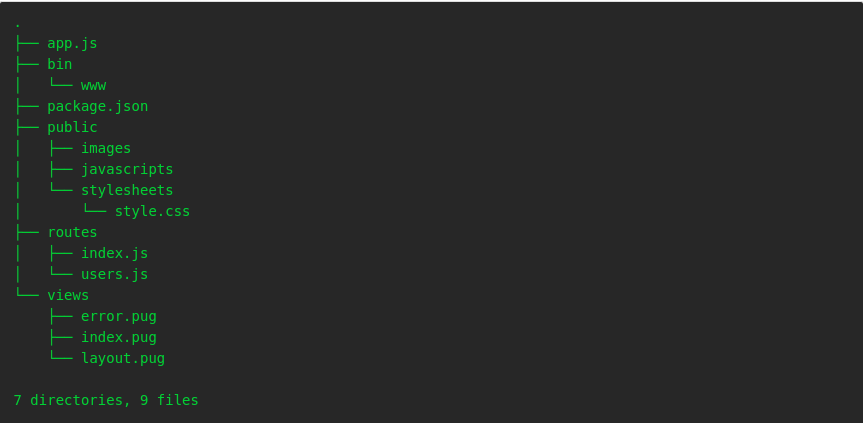
\includegraphics[width=10cm]{./Gambar/express_generator.png}
      \centering
      \caption{Tampilan direktori yang dibuat jika menjalankan express generator.}
      \label{fig:express_generator}
    \end{figure}
    
    Cara menggunakan \textit{express generator} bisa dengan menjalankan \textit{command} ``npx express \{nama file yang akan dibuat\}'' atau bisa dengan \textit{command} ``express \{nama file yang akan dibuat\}'', maka \textit{express generator} akan langsung secara otomatis membuat \textit{folder} dan \textit{file-file} seperti yang ada pada gambar \ref{fig:express_generator}. Pada gambar \ref{fig:express_generator} terdapat sebuah direktori \textit{file} yang berisikan \textit{app.js} yang merupakan \textit{script} utama dari \textit{node.js} yang akan dipanggil ketika perangkat lunak dijalankan, lalu terdapat \textit{folder} \textit{bin} yang digunakan untuk menampung \textit{cache} dari \textit{web application} yang dibangun. Lalu ada \textit{package.json} yang digunakan untuk menyimpan semua nama \textit{library} yang dipakai perangkat lunak. Lalu ada \textit{folder public} yang berfungsi untuk menampung \textit{javascript} dan juga \textit{stylesheet} di dalam perangkat lunak. Terdapat \textit{folder routes} yang berfungsi sebagai \textit{folder} yang menyimpan \textit{script} yang akan digunakan untuk setiap rute yang dipanggil ketika perangkat lunak dijalankan. Lalu ada \textit{folder view} yang merupakan kumpulan dari kode program yang mengurus pada bagian tampilan depan setiap rute dan halaman dari perangkat lunak ketika sudah dijalankan. 
    
    \item {\textit{Routing}}\\
    Fungsi ini berguna untuk memudahkan \textit{web application} untuk bisa menuju kepada halaman yang berbeda dengan memakai \textit{path} dari alamat \textit{url} aplikasi tersebut. Cara menggunakannya adalah dengan menggunakan kode program seperti:
    \begin{lstlisting}
    app.METHOD(PATH, HANDLER)
    \end{lstlisting}
    Kode program seperti itu memiliki arti:
    \begin{itemize}
        \item \textbf{\textit{app}} yang merupakan inisiasi dari \textit{express}.
        \item \textbf{\textit{METHOD}} yang merupakan jenis \textit{http request} dengan menggunakan penggunaan huruf kecil. (\textit{get, post, put,} atau \textit{delete})
        \item \textbf{\textit{PATH}} adalah jalur di dalam \textit{server}.
        \item \textbf{\textit{HANDLER}} adalah fungsi yang akan dieksekusi jika rute yang diakses cocok. 
    \end{itemize}
\end{itemize}

\subsection{Handlebars}\footnote{\url{https://www.npmjs.com/package/handlebars}}
\textit{Handlebars} adalah modul dari \textit{Node.js} yang membantu fungsi penggunaan \textit{template semantic} pada tampilan yang akan digunakan di dalam pembangunan perangkat lunak. \textit{Template semantic} ini membantu pengiriman data \textit{variable} dari \textit{javascript} belakang ke bagian dari \textit{view}. 

\subsection{Simple OAuth2}\footnote{\url{https://www.npmjs.com/package/simple-oauth2}}
Modul ini berguna untuk membantu proses otentikasi pada perangkat lunak yang melakukan otentikasi kepada aplikasi pihak ketiga lainnya. Modul ini membantu perangkat lunak agar bisa menjalankan proses \textit{OAuth}. Pada \textit{simple oauth} ini dapat ditangani 3 alur untuk melakukan otentikasi yaitu:
\begin{itemize}
    \item Alur kode otorisasi\\
    Alur ini dipakai pada aplikasi yang dapat menyimpan data secara persisten. 
    \item \textit{Password Credentials}\\
    Alur ini digunakan pada saat alur sebelumnya tidak dapat dilakukan atau sedang dalam tahap pengembangan. 
    \item \textit{Client Credentials}\\
    \textit{Client} hanya bisa mendapatkan \textit{access token} dengan cara mengirimkan kredensial yang dimiliki oleh \textit{client}. 
\end{itemize}

Untuk bisa menggunakan modul ini, dibutuhkan persyaratan yaitu menggunakan \textit{Node} minimal versi 8. Jika menggunakan \textit{Node} versi 4, 5, atau 6, maka dapat menggunakan \textit{library} \textit{simple-oauth2@1.x}. Cara pemasangan \textit{library} ini dengan cara menuliskan perintah pada \textit{terminal} seperti: 

\begin{lstlisting}
$ npm install --save simple-oauth2
\end{lstlisting}

Saat digunakan, \textit{simple-oauth2} menerima objek yang berisi \textit{parameter} yaitu: 
\begin{itemize}
    \item \textbf{\textit{client}} - objek \textit{parameter} wajib yang memiliki properti: 
    \begin{itemize}
        \item \textbf{\textit{id}} - \textit{Parameter} ini merupakan \textit{parameter} yang dibutuhkan dan diisi dengan menggunakan \textit{client id} dari aplikasi yang sudah didaftarkan. 
        \item \textbf{\textit{secret}} - \textit{Parameter} ini merupakan \textit{parameter} yang dibutuhkan dan diisi dengan menggunakan \textit{client secret} dari aplikasi yang sudah didaftarkan. 
        \item \textbf{\textit{secretParamName}} - Merupakan nama \textit{parameter} yang digunakan untuk mengirimkan \textit{client secret} yang memiliki nilai \textit{default} yaitu \textit{client\_secret} dari aplikasi yang sudah didaftarkan. 
        \item \textbf{\textit{idParamName}} - Merupakan nama \textit{parameter} yang digunakan untuk mengirimkan \textit{client id} yang memiliki nilai \textit{default} yaitu \textit{client\_id} dari aplikasi yang sudah didaftarkan. 
    \end{itemize}
    \item \textbf{\textit{auth}} - objek \textit{parameter} wajib yang memiliki properti: 
    \begin{itemize}
        \item \textbf{\textit{tokenHost}} - \textit{String} yang digunakan untuk mengatur \textit{host} untuk meminta \textit{token} dan merupakan \textit{parameter} yang dibutuhkan.  
        \item \textbf{\textit{tokenPath}} - \textit{String} yang menunjukkan jalur untuk meminta \textit{access token} yang memiliki nilai \textit{default} yaitu ke \textit{/oauth/token}. 
        \item \textbf{\textit{revokePath}} - \textit{String} yang menunjukkan jalur untuk mencabut \textit{access token} yang memiliki nilai \textit{default} yaitu ke \textit{/oauth/revoke}
        \item \textbf{\textit{authorizeHost}} - \textit{String} yang digunakan untuk mengatur \textit{host} untuk meminta \textit{authorization code} dan memiliki nilai \textit{default} yaitu \textit{auth.tokenHost}. 
        \item \textbf{\textit{authorizePath}} - \textit{String} yang menunjukkan jalur untuk meminta \textit{authorization code} yang memiliki nilai \textit{default} yaitu ke \textit{/oauth/authorize}. 
    \end{itemize}
    \item \textbf{\textit{http}} - objek \textit{parameter} yang bersifat opsional yang memiliki fungsi sebagai pengatur opsi \textit{global} ke \textit{internal http library} yang memiliki properti: 
    \begin{itemize}
        \item Semua opsi diperbolehkan kecuali opsi \textit{baseUrl}. Memiliki nilai \textit{default} yaitu \textit{headers.Accept = application/json}. 
    \end{itemize}
    \item \textbf{\textit{options}} - objek \textit{parameter} yang bersifat opsional yang memiliki fungsi sebagai pengatur modul yang memiliki properti: 
    \begin{itemize}
        \item \textbf{\textit{bodyFormat}} - format data yang dikirim dalam \textit{request body} saat mengirimkan \textit{request}. Nilai yang \textit{valid} untuk properti ini adalah \textit{form} atau \textit{json} dan memiliki nilai \textit{default} yaitu \textit{form}. 
        \item \textbf{\textit{authorizationMethod}} - properti yang menunjukkan metode yang dipakai untuk mengirimkan \textit{client.id/client secret} saat meminta \textit{token}. Nilai yang \textit{valid} untuk properti ini adalah \textit{header} atau \textit{body}. Jika properti ini bernilai \textit{body}, maka \textit{bodyFormat} akan dipakai untuk memformat kredensialnya. Nilai \textit{default} dari properti ini adalah \textit{header}.  
    \end{itemize}
\end{itemize}

\begin{lstlisting}
const credentials = {
  client: {
    id: <client-id>,
    secret: <client-secret>,
  },
  auth: {
    tokenHost: 'https://login.microsoftonline.com',
    authorizePath: 'common/oauth2/v2.0/authorize',
    tokenPath: 'common/oauth2/v2.0/token'
  }
};
const oauth2 = require('simple-oauth2').create(credentials);
\end{lstlisting}

\subsubsection{Alur OAuth2 yang Didukung}
Adapun modul ini mendukung beberapa arus \textit{OAuth2} yaitu seperti:
\begin{itemize}
    \item \textit{Authorization Code Flow}\\
    \textit{Authorization Code Flow} ini menjalankan 2 langkah. Langkah pertama yaitu aplikasi akan meminta \textit{permission} kepada pengguna untuk mengakses data mereka. Jika pengguna menyetujui, maka \textit{OAuth2 server} akan mengirimkan \textit{authorization code} kepada pengguna yang dilanjutkan dengan langkah kedua yaitu pengguna mengirimkan \textit{POST request} yang berisi \textit{authorization code} bersamaan dengan \textit{client secret} ke \textit{oauth server} untuk mendapatkan \textit{access token}. 
    
    \item \textit{Password Credentials Flow}\\
    Alur ini menggunakan \textit{username} serta \textit{password} untuk bisa mendapatkan \textit{access token} yang dibutuhkan oleh pengguna. Alur ini biasanya digunakan saat pengguna dengan aplikasi atau sistem operasi dari komputer sudah sangat terpercaya sehingga keamanan \textit{username} dan \textit{password} bisa terjaga. Cara ini biasa dipakai untuk melakukan tes aplikasi secara cepat. 
    
    \item \textit{Client Credentials Flow}\\
    Alur ini cocok untuk pengguna yang melakukan \textit{request} akses ke sumber yang dibawah kontrol dari pengguna itu sendiri. 
\end{itemize}

\subsubsection{Helpers}
Modul ini juga menyediakan sebuah objek pembantu untuk mempermudah proses dari \textit{OAuth2} yaitu:
\begin{itemize}
    \item \textit{Access Token object}\\
    Saat \textit{token} kadaluarsa, diperlukan \textit{refresh token} untuk bisa meminta ulang \textit{access token} yang baru. \textit{Simple OAuth2} menyediakan sebuah kelas \textit{AccessToken} yang memiliki beragam fungsi yang salah satunya membantu mempermudah untuk meminta ulang \textit{access token} saat \textit{token} sudah kadaluarsa. Inisialisasi dari kelas ini seperti 
    
    \begin{lstlisting}
    // Sample of a JSON access token (you got it through
    previous steps)
    const tokenObject = {
      'access_token': '<access-token>',
      'refresh_token': '<refresh-token>',
      'expires_in': '7200'
    };
    \end{lstlisting}
\end{itemize}

\subsection{jsonwebtoken}\footnote{\url{https://www.npmjs.com/package/jsonwebtoken}}
\textit{Jsonwebtoken} merupakan implementasi dari \textit{JSON Web Tokens} yang dikembangkan terhadap \textit{draft-ieft-oauth-json-web-token-08}. \textit{Jsonwebtoken} ini memiliki beberapa fungsi yaitu:
\begin{itemize}
    \item \textbf{jwt.sign(payload,secretOrPrivateKey, [options, callback])}\\
    Fungsi ini bisa berjalan secara \textit{asynchronous} jika \textit{parameter callback} diisi. \textit{Callback} dipanggil dengan \textit{err} atau dengan \textit{JWT}. Tetapi fungsi ini juga bisa berjalan secara \textit{synchronous} dan mengembalikan \textit{JsonWebToken} sebagai sebuah \textit{string}. 
    \item \textbf{jwt.verify(token,secretOrPrivateKey, [options, callback])}\\
    Fungsi ini bisa berjalan secara \textit{asynchronous} jika \textit{parameter callback} diisi. \textit{Callback} dipanggil dengan \textit{payload} yang telah di \textit{decode} jika \textit{signature}-nya \textit{valid} dan ada \textit{parameter} seperti kadaluarsa yang bersifat opsional, \textit{audiens}, atau penerbit akan menjadi \textit{valid}. Jika tidak, maka akan menimbulkan \textit{error}. Fungsi ini juga bisa berjalan secara \textit{synchronous} jika tidak ada \textit{callback} yang diisi. 
    \item \textbf{jwt.decode(token, [options])}\\
    Fungsi ini berjalan secara \textit{synchronous} dan mengembalikan \textit{payload} yang sudah di \textit{decode} tanpa memverifikasi \textit{signature} yang ada \textit{valid} atau tidak. 
\end{itemize}

\textit{Token} yang dipakai pada fungsi \textit{jwt.verify} dan \textit{jwt.decode} adalah \textit{token id} yang didapat dari proses \textit{OAuth} saat melakukan \textit{request access token}. \textit{Token id} biasanya terdiri dari 3 buah komponen penyusun yaitu ada \textit{header, payload,} dan juga \textit{signature}. Berbeda dengan \textit{session id} biasa saat pengguna melakukan \textit{login}, \textit{token id} memiliki bersifat mandiri yang dalam artian memiliki informasi yang lebih kompleks daripada \textit{session id}, sedangkan session id biasanya hanyalah berisi \textit{string} yang panjang dan \textit{random} serta tidak memiliki informasi di dalamnya yang cara kerjanya harus melihat kembali ke tempat penyimpanan data dengan nomor referensi yang adalah \textit{session id}. \textit{Payload} di dalam \textit{token id} menyimpan seluruh informasi mengenai pengguna, sedangkan \textit{signature} berisi status dari \textit{token} tersebut yang bernilai \textit{valid} atau tidaknya. 

\subsection{Isomorphic Fetch}\footnote{\url{https://www.npmjs.com/package/isomorphic-fetch}}
\textit{Isomorphic Fetch} adalah sebuah \textit{polyfill} \textit{window.fetch} untuk digunakan di \textit{node} dan \textit{browserify}. \textit{Polyfill} ini memungkinkan \textit{window.fetch} untuk \textit{javascript engine} yang tidak mendukungnya secara \textit{native}. 

\subsection{Microsoft Graph Client Library}\footnote{\url{https://github.com/microsoftgraph/msgraph-sdk-javascript}}
\textit{Microsoft Graph Client Library} adalah sebuah modul yang disediakan oleh \textit{Microsoft} untuk perangkat lunak yang akan menggunakan \textit{API} ke \textit{Microsoft} bisa lebih mudah. Modul ini hanya sebagai pembungkus dari semua fungsi \textit{API} yang disediakan oleh \textit{Microsoft}. Untuk bisa memakai modul ini, maka harus menginisialisasi terlebih dahulu sebuah objek inisialisasi dari modul ini dengan menggunakan \textit{access token} yang didapat saat melakukan \textit{request} awal. Setelah melakukan inisialisasi, maka setiap \textit{API} dapat diakses dengan menjalankan kode seperti:

\begin{lstlisting}
const result= await client.api(`/me/events`).select('subject,start,end')
            .orderby('start/dateTime DESC').get();
\end{lstlisting}

\textit{API} diatas diisi dengan fungsi yang akan dipanggil lalu \textit{select} diatas diisi dengan data yang akan diambil. \textit{Orderby} digunakan untuk jika data ingin diurutkan berdasarkan urutan tertentu.

\subsection{Slack Web API}\footnote{\url{https://www.npmjs.com/package/@slack/web-api}}
\label{slackWebApi}
Sama seperti \textit{Microsoft Graph Client Library}, \textit{Slack Web API} ini juga adalah modul yang membungkus \textit{method-method} yang disediakan oleh \textit{Slack} agar untuk mengakses \textit{method} bisa lebih mudah. Cara menggunakannya adalah dengan menginisialisasi terlebih dahulu modul yang akan dipakai sebagai kelas, lalu menginisialisasi kelas ke sebuah \textit{variable} yang diisikan dengan \textit{parameter slack access token} yang didapat dari \textit{request}. Setelah itu, jalankan \textit{variable} tersebut dengan memanggil \textit{scope} yang dipakai seperti contoh pada kode:

\begin{lstlisting}
const web = new WebClient(slack_access_token);

  const result = await web.users.profile.set({
    "profile":{
        "status_text": "In A Meeting",
        "status_emoji": ":no_entry:"
      }
  });
\end{lstlisting}

Untuk setiap \textit{scope} yang dipakai akan memerlukan \textit{request body} yang berbeda-beda. Untuk mengetahui \textit{request body} yang diperlukan, dapat dilihat pada \url{https://api.slack.com/methods}. 

\section{\textit{Heroku}}
\textit{Heroku} adalah \textit{cloud platform} yang menampung program agar bisa dibangun, dan dijalankan di \textit{cloud}.\cite{heroku} \textit{Heroku} mendukung beberapa bahasa pemrograman yaitu: \textit{Ruby, Node.js, Java, Python, Clojure, Scala, Go, }dan \textit{PHP}. 
\subsection{Dyno}
\textit{Dyno} adalah sebuah wadah berbasis \textit{Unix} yang disediakan oleh \textit{Heroku}. \textit{Dyno} disini dikategorikan ke 3 jenis \textit{dyno} yaitu:
\begin{itemize}
    \item \textit{Web Dyno} \\ 
    \textit{Web dyno} adalah \textit{dyno} yang berjalan pada tipe proses \textit{web}. \textit{Web dyno} adalah satu-satunya \textit{dyno} yang bisa menerima \textit{HTTP} dari \textit{router heroku}. 
    \item \textit{Worker Dyno} \\ 
    \textit{Worker dyno} adalah \textit{dyno} yang berjalan selain pada tipe proses \textit{web}. \textit{Worker dyno} biasa digunakan untuk pekerjaan pada latar belakang, sistem antrian, dan pekerjaan berjangka waktu tertentu. 
    \item \textit{One-off Dyno} \\ 
    \textit{One-off dyno} adalah \textit{dyno} yang bersifat sementara dan contoh penggunaannya adalah seperti saat migrasi basis data. \textit{Dyno} ini dijalankan menggunakan \textit{command shell}. 
\end{itemize}
\textit{Heroku} menyediakan beberapa paket \textit{dyno} yang mempengaruhi karakteristik dan juga cara kerja \textit{dyno} seperti:
\begin{itemize}
    \item \textit{Free} \\ 
    Pada paket ini, jumlah \textit{dyno} yang didapat untuk setiap \textit{proccess type} adalah 1 serta adanya batasan \textit{dyno hours} yaitu sebanyak 550 jam untuk akun yang belum terverifikasi dan 1000 jam untuk akun yang sudah terverifikasi. \textit{Dyno} akan memasuki kondisi \textit{sleep} jika \textit{web dyno} sedang tidak aktif selama lebih dari 30 menit. \textit{Dyno} akan kembali lagi aktif ketika ada arus yang masuk ke \textit{HTTP} tetapi ada keterlambatan untuk memproses arus tersebut.  
    \item \textit{Hobby} \\ 
    Jumlah \textit{dyno} yang didapat untuk setiap \textit{proccess type} adalah 1. Jumlah \textit{dyno hours} di dalam paket ini tidak dibatasi tetapi setiap \textit{dyno hours} yang dipakai akan dikenakan biaya sebesar \$7 per jam per bulannya.  
    \item \textit{Standard} \\
    Jumlah \textit{dyno} yang didapat untuk setiap \textit{proccess type} adalah sebanyak 10. Jumlah \textit{dyno} yang bisa dijalankan secara bersamaan adalah sebanyak 100 pada satu aplikasi. Harga dari \textit{dyno hours} berkisar antara \$25 sampai \$500. 
    \item \textit{Performance} \\
    Jumlah \textit{dyno} yang didapat untuk setiap \textit{proccess type} adalah sebanyak 10. Jumlah \textit{dyno} yang bisa dijalankan secara bersamaan adalah sebanyak 100 pada satu aplikasi. Harga dari \textit{dyno hours} berkisar antara \$25 sampai \$500. Perbedaan dari paket \textit{standard} dengan paket \textit{performance} adalah paket ini bersifat \textit{dedicated}. 
\end{itemize}

Pada \textit{heroku} terdapat banyak fitur penyokong untuk menjalankan aplikasi seperti basis data, sistem antrean, layanan \textit{email}, dan lain-lain yang disebut dengan \textit{add-ons}. Daftar dari \textit{add-ons} yang tersedia untuk \textit{Heroku} dapat dilihat pada situs \textit{web} \textit{Elements Marketplace} (\url{https://elements.heroku.com/addons}) Beberapa contoh \textit{add-ons} yang tersedia di \textit{heroku} antara lain:

\subsection{Heroku Scheduler}
\textit{Scheduler} adalah \textit{add-ons} gratis yang bertugas untuk mengatur jalannya pekerjaan dalam aplikasi secara berkala sesuai dengan \textit{interval} yang ditentukan oleh pengguna. Tugas \textit{heroku scheduler} lebih mirip dengan cara kerja \textit{cron} di \textit{server} tradisional. Melalui \textit{scheduler}, pekerjaan dimungkinkan untuk dijalankan setiap 10 menit sekali, setiap jam, setiap hari, atau pada waktu yang ditentukan. Saat dijalankan, \textit{job} ini akan berjalan sebagai \textit{one-off dynos} dan akan muncul di dalam \textit{logs} sebagai \textit{dyno} seperti \textit{scheduler.X}. Cara memasang \textit{add-ons} ini melalui \textit{command shell} adalah dengan cara:
\begin{lstlisting}
\$ heroku addons:create scheduler:standard
\end{lstlisting}
\textit{Scheduler} akan menjalankan \textit{one-off dynos} yang akan dihitung sebagai penggunaan dari pengguna pada bulan itu. \textit{Dyno-hours} yang dihitung akan sama seperti saat menjalankan aplikasi atau dari \textit{dynos} yang berskala. Untuk pemakaian dari \textit{dyno-hours} dapat pengguna lihat pada bagian tagihan pada tab ``\textit{Manage account}''. 

\subsection{\textit{Heroku Postgres}}
\textit{Heroku Postgres} adalah layanan basis data SQL yang dikelola dan disediakan langsung oleh \textit{Heroku}. Basis data \textit{Heroku Postgres} dapat diakses dengan menggunakan semua bahasa pemrograman dengan \textit{driver PostgreSQL} termasuk seluruh bahasa pemrograman yang didukung di \textit{Heroku}. Untuk cara penggunaannya di dalam bahasa \textit{Node.js}, maka dibutuhkan langkah-langkah yaitu 
\begin{itemize}
    \item Melakukan pemasangan modul pg sebagai \textit{dependency} dengan cara menjalankan \textit{command line} seperti:
    \begin{lstlisting}
    $ npm install pg 
    \end{lstlisting}
    \item Melakukan koneksi ke \textit{url} dari basis data yang disediakan oleh \textit{Heroku} saat perangkat lunak dijalankan. Contoh dari kode programnya seperti:
    \begin{lstlisting}
    const { Client } = require('pg');

    const client = new Client({
      connectionString: database_url,
      ssl: true,
    });
    
    client.connect();
    
    client.query('SELECT table_schema,table_name FROM
    information_schema.tables;', (err, res) => {
      if (err) throw err;
      for (let row of res.rows) {
        console.log(JSON.stringify(row));
      }
      client.end();
    });
    \end{lstlisting}
\end{itemize}
